\documentclass[11pt,a4paper,sans]{moderncv} % Font sizes: 10, 11, or 12; paper sizes: a4paper, letterpaper, a5paper, legalpaper, executivepaper or landscape; font families: sans or roman

\moderncvstyle{banking} % CV theme - options include: 'casual' (default), 'classic', 'oldstyle' and 'banking'
\moderncvcolor{grey} % CV color - options include: 'blue' (default), 'orange', 'green', 'red', 'purple', 'grey' and 'black'

\usepackage[scale=0.75]{geometry} % Reduce document margins
%\setlength{\hintscolumnwidth}{3cm} % Uncomment to change the width of the dates column
%\setlength{\makecvtitlenamewidth}{10cm} % For the 'classic' style, uncomment to adjust the width of the space allocated to your name

%\usepackage{hyperref}
\usepackage{graphicx}

\usepackage{subcaption}
\usepackage{tikz}
\usetikzlibrary{arrows,automata,positioning}

\title{Research Plan}

\firstname {Sreejith}
\familyname {A V}

\begin{document}
\makecvtitle % Print the CV title

\section{Introduction}
My research lies at the intersection of theoretical computer science and practical applications, focusing on logic, automata theory, and their integration into fields such as formal verification and, more recently, machine learning. I completed my Ph.D. under the supervision of Prof. Kamal Lodaya at the Institute of Mathematical Sciences, Chennai, and postdoctoral research at prestigious institutions, including IRIF (France), the University of Warsaw (Poland), TIFR and CMI. I joined IIT Goa as an Assistant Professor and currently serve as an Associate Professor. \\


My Ph.D. thesis earned an \emph{ACM India Honorable Mention} in 2014, recognizing its contributions to descriptive complexity. At IIT Goa, I have mentored Ph.D. and master's students and secured competitive funding from agencies such as CEFIPRA, SERB and MoES.\\

My early research centered on the theoretical foundations of logic and automata. Over time, I expanded into applied research.
This document outlines my research journey, highlighting key contributions, ongoing projects, and future directions.
\section{Descriptive Complexity: Ph.D.}
Logic provides a precise framework to express mathematical properties unambiguously. It plays a vital role in areas like descriptive complexity~\cite{immerman_book}, and set theory~\cite{ject_setTheory}.
%While Hilbert's program sought to axiomatize mathematics, Gödel's incompleteness theorem underscored the limits of formal systems \cite{godel_incompleteness}. Yet, l
Logic has driven advances among other things in formal verification, database, and artificial intelligence~\cite{vardi_logicEffectiveness}.

\subsection{Contributions}
Our work introduced modulo counting operators, thereby enhancing the expressiveness of logics. Key contributions (see my thesis \cite{sav_thesis}) include:
\begin{enumerate}
 \item Extending Linear temporal logic (\textsf{LTL}) with modulo counting operators, enhancing its expressiveness while retaining PSPACE complexity for model checking~\cite{my_ltlmod,my_ltlsuccinct}.
 \item Resolving an \emph{open problem} in circuit complexity by showing that certain regular languages are not definable in first-order logic with addition and modulo counting operators~\cite{my_foplus}. It connects logic and semigroup theory to show strict hierarchies in some circuit complexity classes.
\end{enumerate}

\subsection{Awards and Recognition}
\begin{itemize}
    \item \textbf{ACM India Honorable Mention (2014):} Ph.D. thesis titled \emph{Regular Quantifiers in Logics}.
\end{itemize}

\section{Countable Words: Postdoctoral and IIT Goa}
This work is at the meeting point of two important branches of language theory:
\begin{enumerate}
 \item \textbf{Extension of finite word language theories:} This branch explores structures beyond finite words, such as infinite words~\cite{Buchi62} and infinite trees~\cite{Rabin69}.
 \item \textbf{Characterization of logics:} This branch focuses on identifying and classifying logics, with First-order logic~\cite{Schutzenberger65} serving as a key example.
\end{enumerate}

We study countable words, the largest extension that is known to have a theory of recognizability.

\subsection{Contributions}
Our work \cite{icalp15} provided the first algebraic characterizations of intermediate logics. We:
\begin{itemize}
    \item Developed characterizations (algebraic / regular expression) for various natural restrictions and extensions of first-order logic like \textsf{FO}$^2$ and weak \textsf{MSO}~\cite{icalp15,ms16}.
    \item Established decomposition theorems for algebraic structures in this context~\cite{lics19,jcss23}.
    \item Demonstrated that certain logics, like weak \textsf{MSO}, cannot be decomposed using a finite set~\cite{fct21}.
\end{itemize}
These results provide mathematical tools for comparing expressiveness among logics.

\subsection{Achievements}
\begin{itemize}
    \item \textbf{Supervision:} Informally co-superviced Saptarshi Sarkar (Ph.D. under Bharat Adsul, IIT Bombay).
\end{itemize}


\section{One-Counter Automata: IIT Goa}
Finite automata models complex systems, from computational processes \cite{vardi95} to biological phenomena \cite{Barto75}. Deterministic one-counter automata (DOCA) extend finite automata with an integer counter, enabling the modeling of certain infinite-state systems (see Figure 1). DOCAs are strictly more expressive than finite automata, making them promising candidates for replacing finite automata in applications, provided scalable algorithms can be developed. This research aims to advance the understanding and applicability of DOCAs.

\subsection{Contributions}
We addressed two key problems:
\begin{itemize}
    \item \textbf{Equivalence of weighted DOCA:} We showed decidability for a large subclass using novel reachability techniques, placing the problem in P \cite{fsttcs23,icla25}. The equivalence problem for the full class remains a fundamental open problem.
    \item \textbf{Active learning algorithms for DOCAs:}
    \begin{itemize}
    \item Developed SAT-based algorithm~\cite{learning24} that is better than state of the art \cite{gaetan}.
    \item Developed the first polynomial-time algorithm (yet to be published), improving on the current complexity of $P^{NP}$. This work will enable faster and more efficient learning of DOCAs.
    \end{itemize}
\end{itemize}

\subsection{Achievements}
\begin{itemize}
    \item \textbf{Funding:} SERB research grant for \emph{Probabilistic Pushdown Automata} (2021--2024).
    \item \textbf{Supervision:} Prince Mathew (Ph.D. student), expected to submit thesis by Dec 2024.
\end{itemize}
\begin{minipage}{\textwidth}
\begin{center}
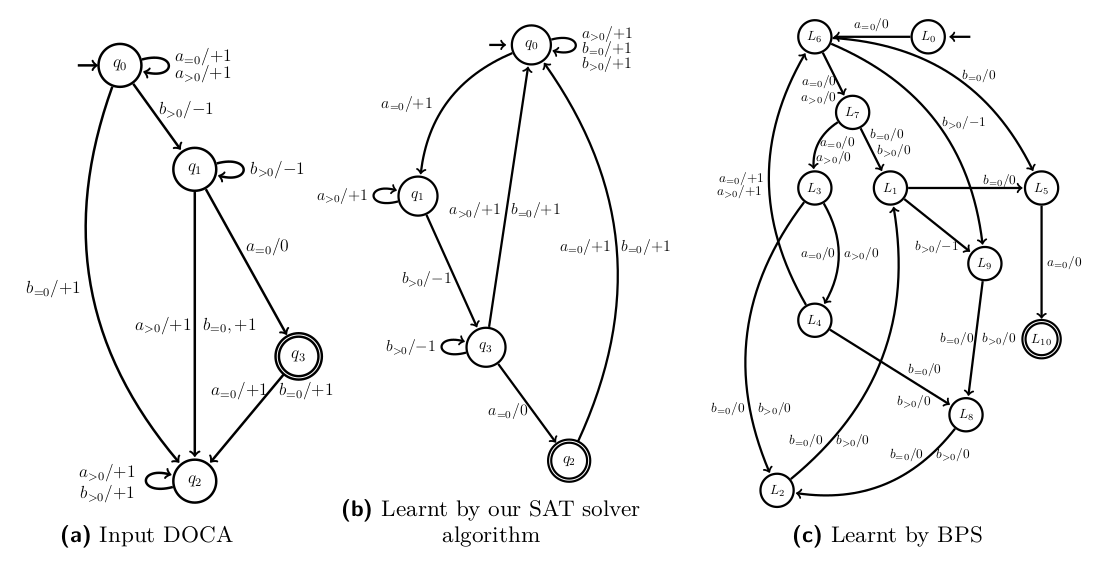
\includegraphics[width=0.66\textwidth]{doca.png} \\
\textbf{Figure 1} The input DOCA recognizes the language $\{a^nb^na ~|~ n > 0\}$.
\end{center}
\end{minipage}

\section{Water Research Using Geostationary Data}
In collaboration with environmental scientists, we developed methods to estimate river water discharge (see Figure 2.) using geospatial data (along with in-situ measurements) \cite{esd21}. Ongoing work focuses on soil moisture estimation, contributing to water resource management.

\subsection{Achievements}
\textbf{Funding:} Ministry of Earth Science (MoES) sanctioned project \emph{Remote sensing based method
for detecting water discharge in the Ganga and Brahmaputra rivers} is completed

\begin{minipage}{\textwidth}
\begin{center}
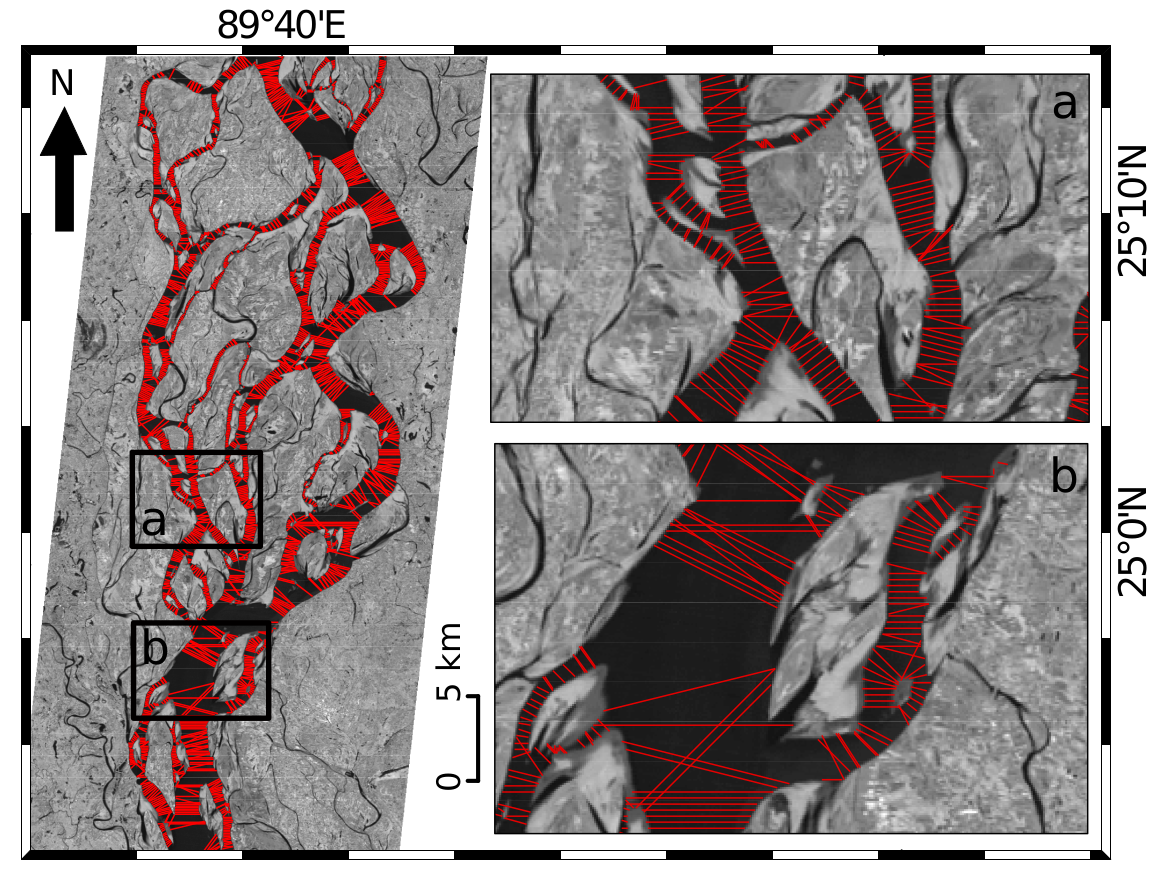
\includegraphics[width=0.51\textwidth]{river-width.png} \\
  \textbf{Figure 2} River width estimation.
\end{center}
\end{minipage}


\section{Formal Methods in Machine Learning: Future Directions}
Adaptive control systems used in safety-critical applications, such as autonomous vehicles and robotics, demand rigorous safety verification. Traditional verification methods face significant challenges when these systems incorporate machine learning algorithms for decision-making.\\

Our research aims to address these challenges by employing formal verification techniques, including abstraction and SAT/SMT solvers, to ensure the safety and reliability of such systems.

\subsection{Future directions}
\begin{itemize}
 \item Developing scalable verification techniques for machine learning models.
 \item Developing verification techniques for control systems that use machine learning algorithms inside.
\end{itemize}

\subsection{Achievements}
\begin{itemize}
    \item \textbf{Funding:} Indo-French grant (CEFIPRA) for \emph{Formal Verification of Adaptive Control Algorithms}.
    \item \textbf{Visiting Faculty and Funding:} University of Bordeaux, contributing to research on \emph{Formal methods in machine learning}.
\end{itemize}



\section{Conclusion}
My research combines theoretical rigor with practical applications, advancing the fields of logic, automata theory, and their applications in formal verification. In the next five years, I aim to:
\begin{itemize}
    \item Continue the foundational work in automata theory and logic.
    \item Design and develop algorithms and tools for formal verification of machine learning systems.
    \item Expand interdisciplinary collaborations, applying theoretical methods to water research.
\end{itemize}


\bibliographystyle{alpha}
\bibliography{papers}

\end{document}
